\documentclass{article}
\usepackage{tikz}
\usetikzlibrary{matrix,shapes,arrows,positioning,chains,patterns,fit,decorations.pathreplacing,calc,plotmarks}
\tikzset{
    dotted_block/.style={
        draw=black!30!white, 
        dashed,
        inner ysep=2mm,
        inner xsep=10mm, 
        rectangle, 
        rounded corners
    },
    block/.style={
        draw,
        rectangle,
        rounded corners,
        minimum height=2em,
        minimum width=2em
    },
    operator/.style={
        draw,
        circle,
        thin,
        minimum height=1em,
	   inner sep=1pt
    },
    weight/.style={
        draw,
        thin,
        rounded corners,
        rectangle,
        %minimum height=2em,
        %minimum width=4em
    },
    value/.style={
        draw,
        thin,
        rectangle,
        %minimum height=2em,
        %minimum width=3em
    },
    gain/.style={
        regular polygon, 
        regular polygon sides=3,
        draw, 
        fill=white, 
        text width=1em,
        inner sep=1mm, 
        outer sep=0mm,
        shape border rotate=-90
    },
    concat/.style={
        draw,
        shape=circle, 
        fill=black,
        %minimum height=0.5em,
	   inner sep=0pt
    },
}
\usepackage{pgfplots}
\pgfplotsset{compat=1.17}

\begin{document}

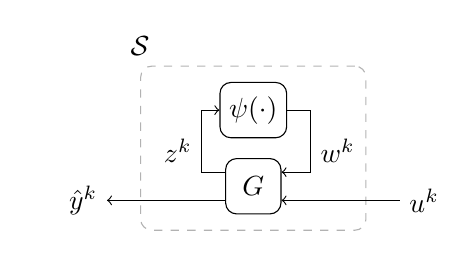
\begin{tikzpicture}[node distance = 0.25cm and 0.7cm, auto, align=center]

    % blocks
    \node[] (output) {};
    \node[block, right= of output] (G) {$G$};
    \node[block, above= of G] (delta) {$\psi(\cdot)$};
    \node[right= of G] (input) {};
    \node[dotted_block, fit = (G) (delta)] (S) {};
    \node at (S.north west) [above] {$\mathcal{S}$};
    
    
    % Input and outputs coordinates
    \coordinate[] (outputz)  at ($(G.south west)!0.75!(G.north west)$);
    \coordinate[] (outputy)  at ($(G.south west)!0.25!(G.north west)$);
    \coordinate[] (inputw) at ($(G.south east)!0.75!(G.north east)$);
    \coordinate[] (inputu) at ($(G.south east)!0.25!(G.north east)$);
    
    % lines
    \draw[<-] (inputu) -- ++(1.5,0);
    \draw[-] (inputu) ++(1.5,0) node[right]{$u^k$}++(0.5,0);
    \draw[->] (outputz) -- ++(-0.3,0) node[above left]{$z^k$}  |-   (delta.west) ;
    \draw[->] (outputy)  --  ++(-1.5,0);
    \draw[-] (outputy)  ++(-1.5,0) node[left]{$\hat{y}^k$} ++(-1,0);
    \draw[->] (delta.east)  -- ++(0.3,0) |- node[above right] {$w^k$}(inputw) ;

\end{tikzpicture}

\end{document}